\documentclass{beamer}
%\documentclass[handout]{beamer}
\usepackage[latin1]{inputenc}


%%%%%%%%%%%%%
%% THEMES w/o navigaton
%\usetheme{default}
%\usetheme{Madrid}
%\usetheme{Pittsburgh}
\usetheme{Boadilla}

%%%%%%%%%%%%%
%% THEMES w/ tree navigation
%\usetheme{Antibes}

%%%%%%%%%%%%%
%% THEMES w/ TOC sidebar
%\usetheme{Berkeley}

%%%%%%%%%%%%%
%% THEMES w/ miniframe navigation
%\usetheme{Berlin}
%\usetheme{Darmstadt}
%\usetheme{Ilmenau}
%\usetheme{Singapore}
%\usetheme{Frankfurt}

%%%%%%%%%%%%%
%% THEMES w/ section/subsection titles
%\usetheme{Copenhagen}
%\usetheme{Warsaw}


%%%%%%%%%%%%%%%

\usecolortheme{beaver}

\usepackage{tikz}
\usetikzlibrary{arrows}

\DeclareMathOperator*{\argmax}{arg\,max}
\DeclareMathOperator*{\argmin}{arg\,min}
%\DeclareMathOperator*{\Em}{E_w(x=x^{(m)},h)}
\DeclareMathOperator*{\Em}{E_w(x^{(m)},h)}
\DeclareMathOperator*{\E}{E_w(x,h)}
\DeclareMathOperator*{\Es}{E(x,h)}
%\DeclareMathOperator*{\nw}{\nabla_{w_{ij}}}
\DeclareMathOperator*{\nw}{\partial_{w_{ij}}}
\newcommand{\btheta}{\boldsymbol \theta }
\newcommand{\bi}{\begin{itemize}}
\newcommand{\ei}{\end{itemize}}
\newcommand{\be}{\begin{enumerate}}
\newcommand{\ee}{\end{enumerate}}


\setbeamertemplate{footline}{\hfill\insertframenumber/\inserttotalframenumber}
%\setbeamertemplate{footline}[page number]

\makeatletter
\def\blfootnote{\xdef\@thefnmark{}\@footnotetext}
\makeatother

\title[Deep Learning]{Deep Learning \& Neural Networks\\Lecture 2}
\author[K. Duh]{Kevin Duh}
\institute[]{Graduate School of Information Science\\Nara Institute of Science and Technology}
\date{Jan 16, 2014}

\begin{document}

\begin{frame}[plain]
\titlepage
\end{frame}


\AtBeginSubsection[]{
\begin{frame}
\frametitle{Today's Topics}
\tableofcontents[currentsection]
\end{frame}
}



%%%%%%%%%
\begin{frame}
\frametitle{Today's Topics}
\tableofcontents
\end{frame}

%SECTION%%%%%%%%%%%%%%%%%%%
\section{General Ideas in Deep Learning}
%%%%%%%%%%%%%%%%%%%%

%% SUBSECTION%%%%%
\subsection[Why Hard]{Motivation for Deep Architectures and why is it hard?}


%%%%%%%%%%%%%%%%
\begin{frame}
\frametitle{The Promise of Deep Architectures}
\begin{columns}
\begin{column}{0.5\textwidth}
\centerline{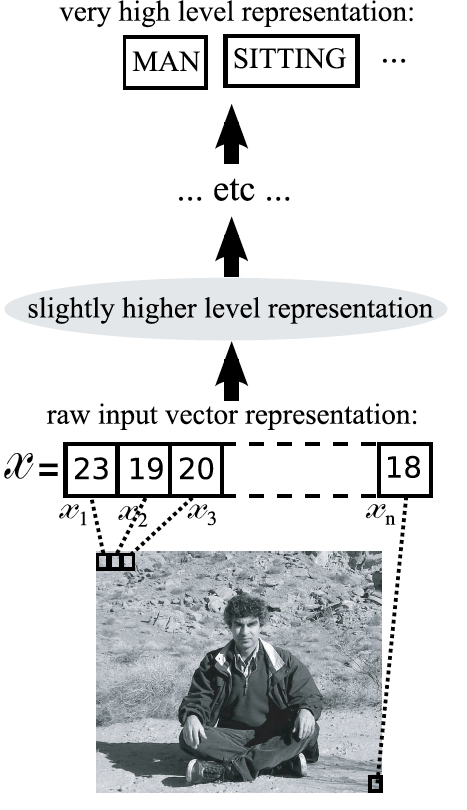
\includegraphics[scale=0.3]{figs/bengio_sitting}}
\end{column}
\begin{column}{0.5\textwidth}
\bi
\item \textit{Understanding in AI} requires high-level abstractions, modeled by highly non-linear functions
\pause
\item These abstractions must disentangle factors of variation in data (e.g.~3D pose, lighting)
\pause
\item Deep Architecture is one way to achieve this: each intermediate layer is a successively higher level abstraction
\ei
\textit{(*Example from \cite{bengio09book})}
\end{column}
\end{columns}
\end{frame}


%%%%%%%%%%%%%%%%
\begin{frame}
\frametitle{The Promise of Deep Architectures}
\begin{columns}
\begin{column}{0.5\textwidth}
\centerline{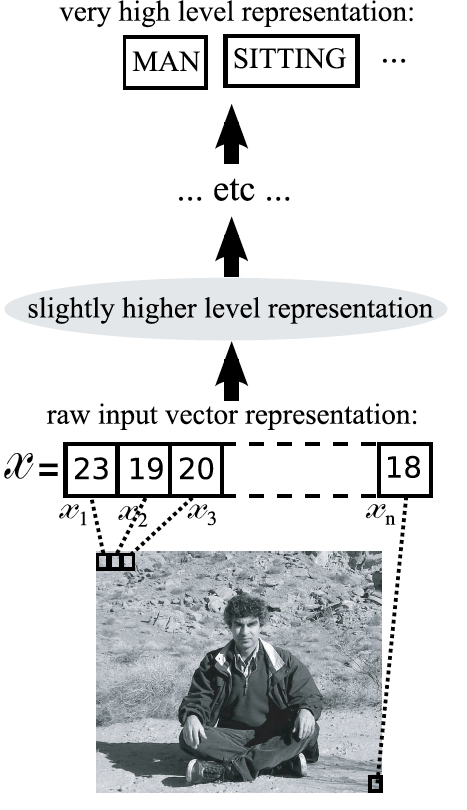
\includegraphics[scale=0.3]{figs/bengio_sitting}}
\end{column}
\begin{column}{0.5\textwidth}
\begin{center}
\begin{tikzpicture}[-,>=stealth',shorten >=1pt,auto,node distance=3cm,
  thick,main node/.style={circle,fill=blue!20,draw,font=\sffamily\Large\bfseries}]

  \node[main node] (x1) at (0,0) {$x_1$};
  \node[main node] (x2) at (2,0) {$x_2$};
  \node[main node] (x3) at (4,0) {$x_3$};
  \node[main node] (h1) at (0,2) {$h_1$};
  \node[main node] (h2) at (2,2) {$h_2$};
  \node[main node] (h3) at (4,2) {$h_3$};
  \node[main node] (h'1) at (0,4) {$h'_1$};
  \node[main node] (h'2) at (2,4) {$h'_2$};
  \node[main node] (h'3) at (4,4) {$h'_3$};
  \node[main node] (y) at (2,6) {$y$};

  \path[every node/.style={font=\sffamily\small}]
    (x1) edge node {} (h1)
    (x1) edge node {} (h2)
    (x1) edge node {} (h3)
    (x2) edge node {} (h1)
    (x2) edge node {} (h2)
    (x2) edge node {} (h3)
    (x3) edge node {} (h1)
    (x3) edge node {} (h2)
    (x3) edge node {} (h3)
    (h1) edge node {} (h'1)
    (h1) edge node {} (h'2)
    (h1) edge node {} (h'3)
    (h2) edge node {} (h'1)
    (h2) edge node {} (h'2)
    (h2) edge node {} (h'3)
    (h3) edge node {} (h'1)
    (h3) edge node {} (h'2)
    (h3) edge node {} (h'3)
    (h'1) edge node {} (y)
    (h'2) edge node {} (y)
    (h'3) edge node {} (y) ;

\end{tikzpicture}
\end{center}
\end{column}
\end{columns}
\end{frame}


%%%%%%%%%%%%%%%%
\begin{frame}
\frametitle{Why are Deep Architectures hard to train?}
\begin{columns}
\begin{column}{0.5\textwidth}
Vanishing gradient problem in Backpropagation
\bi
\item $ \frac{\partial Loss}{ \partial w_{ij}} = {\color{red} \frac{\partial Loss}{ \partial in_j}} {\color{blue} \frac{ \partial in_j}{ \partial w_{ij}}}  = {\color{red} \delta_j}x_i$
\item ${\color{red} \delta_j =  \left[\sum_{j+1} \delta_{j+1} w_{j(j+1)}\right] \sigma'(in_j)}$
\item ${\color{red} \delta_j}$ may vanish after repeated multiplication
\ei
\end{column}
\begin{column}{0.5\textwidth}
\begin{center}
\begin{tikzpicture}[-,>=stealth',shorten >=1pt,auto,node distance=3cm,
  thick,main node/.style={circle,fill=blue!20,draw,font=\sffamily\Large\bfseries}]

  \node[main node] (x1) at (0,0) {$x_1$};
  \node[main node] (x2) at (2,0) {$x_2$};
  \node[main node] (x3) at (4,0) {$x_3$};
  \node[main node] (h1) at (0,2) {$h_1$};
  \node[main node] (h2) at (2,2) {$h_2$};
  \node[main node] (h3) at (4,2) {$h_3$};
  \node[main node] (h'1) at (0,4) {$h'_1$};
  \node[main node] (h'2) at (2,4) {$h'_2$};
  \node[main node] (h'3) at (4,4) {$h'_3$};
  \node[main node] (y) at (2,6) {$y$};

   \node(wij) at (4.3,1) {${\color{red}w_{ij}}$};
   \node(wjj1) at (4.6,3) {${\color{red}w_{j(j+1)}}$};
   
  \path[every node/.style={font=\sffamily\small}]
    (x1) edge node {} (h1)
    (x1) edge node {} (h2)
    (x1) edge node {} (h3)
    (x2) edge node {} (h1)
    (x2) edge node {} (h2)
    (x2) edge node {} (h3)
    (x3) edge node {} (h1)
    (x3) edge node {} (h2)
    (x3) edge node {} (h3)
    (h1) edge node {} (h'1)
    (h1) edge node {} (h'2)
    (h1) edge node {} (h'3)
    (h2) edge node {} (h'1)
    (h2) edge node {} (h'2)
    (h2) edge node {} (h'3)
    (h3) edge node {} (h'1)
    (h3) edge node {} (h'2)
    (h3) edge node {} (h'3)
    (h'1) edge node {} (y)
    (h'2) edge node {} (y)
    (h'3) edge node {} (y) ;

\end{tikzpicture}
\end{center}
\end{column}
\end{columns}
\end{frame}



%%%%%%%%%%%%%%%%
\begin{frame}
\frametitle{Empirical Results: Poor performance of Backpropagation\\ on Deep Neural Nets \cite{erhan09difficulty}}
\bi
\item MNIST digit classification task; 400 trials (random seed)
\item Each layer: initialize $w_{ij}$ by uniform$[-1/\sqrt{(FanIn)}, 1/\sqrt{(FanIn)}]$
\item Although $L+1$ layers is more expressive, worse error than $L$ layers
\ei 
\centerline{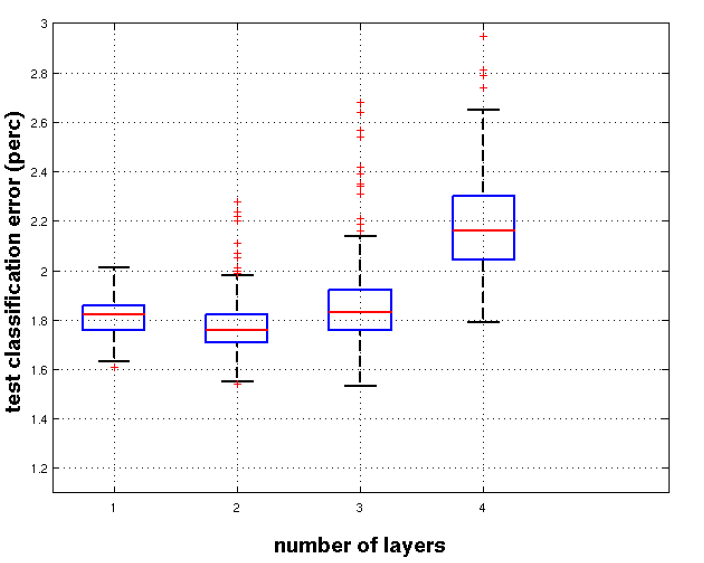
\includegraphics[scale=0.31]{figs/difficulty_backprop}}
\end{frame}

%%%%%%%%%%%%%%%%
\begin{frame}
\frametitle{Local Optimum Issue in Neural Nets}
\bi
\item For 2-Layer Net and more, the training objective is not convex, so different local optima may be achieved depending on initial point
\item For Deep Architectures, Backpropagation is apparently getting a local optimum that does not generalize well
\ei
\centerline{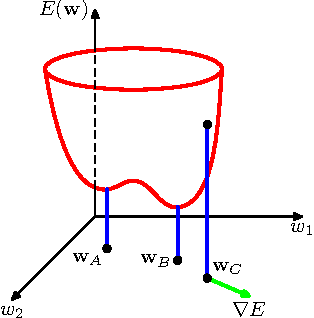
\includegraphics[scale=0.9]{figs/local_optimum}}
\blfootnote{*Figure from Chapter 5, \cite{bishopPRML}}
\end{frame}

%% SUBSECTION%%%%%
\subsection[Breakthrough]{Main Breakthrough in 2006: Layer-wise Pre-Training}

%%%%%%%%%%%%%%%%
\begin{frame}
\frametitle{Layer-wise Pre-training \cite{hinton06dbn}}
First, train one layer at a time, optimizing data-likelihood objective $P(x)$
\begin{center}
\begin{tikzpicture}[-,>=stealth',shorten >=1pt,auto,node distance=3cm,
  thick,main node/.style={circle,fill=blue!20,draw,font=\sffamily\Large\bfseries}]

  \node[main node] (x1) at (0,0) {$x_1$};
  \node[main node] (x2) at (2,0) {$x_2$};
  \node[main node] (x3) at (4,0) {$x_3$};
  \node[main node] (h1) at (0,2) {$h_1$};
  \node[main node] (h2) at (2,2) {$h_2$};
  \node[main node] (h3) at (4,2) {$h_3$};
  \node[main node] (h'1) at (0,4) {$h'_1$};
  \node[main node] (h'2) at (2,4) {$h'_2$};
  \node[main node] (h'3) at (4,4) {$h'_3$};
  \node[main node] (y) at (2,6) {$y$};

  \draw[blue,ultra thick,-latex,<->] (5,0) -- node[right]{Train Layer1} (5,2);


  \path[every node/.style={font=\sffamily\small}]
    (x1) edge node {} (h1)
    (x1) edge node {} (h2)
    (x1) edge node {} (h3)
    (x2) edge node {} (h1)
    (x2) edge node {} (h2)
    (x2) edge node {} (h3)
    (x3) edge node {} (h1)
    (x3) edge node {} (h2)
    (x3) edge node {} (h3)
    (h1) edge node {} (h'1)
    (h1) edge node {} (h'2)
    (h1) edge node {} (h'3)
    (h2) edge node {} (h'1)
    (h2) edge node {} (h'2)
    (h2) edge node {} (h'3)
    (h3) edge node {} (h'1)
    (h3) edge node {} (h'2)
    (h3) edge node {} (h'3)
    (h'1) edge node {} (y)
    (h'2) edge node {} (y)
    (h'3) edge node {} (y) ;

\end{tikzpicture}
\end{center}
\end{frame}


%%%%%%%%%%%%%%%%
\begin{frame}
\frametitle{Layer-wise Pre-training \cite{hinton06dbn}}
First, train one layer at a time, optimizing data-likelihood objective $P(x)$
\begin{center}
\begin{tikzpicture}[-,>=stealth',shorten >=1pt,auto,node distance=3cm,
  thick,main node/.style={circle,fill=blue!20,draw,font=\sffamily\Large\bfseries}]

  \node[main node] (x1) at (0,0) {$x_1$};
  \node[main node] (x2) at (2,0) {$x_2$};
  \node[main node] (x3) at (4,0) {$x_3$};
  \node[main node] (h1) at (0,2) {$h_1$};
  \node[main node] (h2) at (2,2) {$h_2$};
  \node[main node] (h3) at (4,2) {$h_3$};
  \node[main node] (h'1) at (0,4) {$h'_1$};
  \node[main node] (h'2) at (2,4) {$h'_2$};
  \node[main node] (h'3) at (4,4) {$h'_3$};
  \node[main node] (y) at (2,6) {$y$};

  \draw[blue,ultra thick,-latex,<->] (5,2) -- node[right]{Train Layer2} (5,4);
  \draw[blue,ultra thick,-latex,<->] (5,0) -- node[right]{Keep Layer1 fixed} (5,2);

  \path[every node/.style={font=\sffamily\small}]
    (x1) edge node {} (h1)
    (x1) edge node {} (h2)
    (x1) edge node {} (h3)
    (x2) edge node {} (h1)
    (x2) edge node {} (h2)
    (x2) edge node {} (h3)
    (x3) edge node {} (h1)
    (x3) edge node {} (h2)
    (x3) edge node {} (h3)
    (h1) edge node {} (h'1)
    (h1) edge node {} (h'2)
    (h1) edge node {} (h'3)
    (h2) edge node {} (h'1)
    (h2) edge node {} (h'2)
    (h2) edge node {} (h'3)
    (h3) edge node {} (h'1)
    (h3) edge node {} (h'2)
    (h3) edge node {} (h'3)
    (h'1) edge node {} (y)
    (h'2) edge node {} (y)
    (h'3) edge node {} (y) ;

\end{tikzpicture}
\end{center}
\end{frame}

%%%%%%%%%%%%%%%%
\begin{frame}
\frametitle{Layer-wise Pre-training \cite{hinton06dbn}}
Finally, fine-tune labeled objective $P(y|x)$ by Backpropagation
\begin{center}
\begin{tikzpicture}[-,>=stealth',shorten >=1pt,auto,node distance=3cm,
  thick,main node/.style={circle,fill=blue!20,draw,font=\sffamily\Large\bfseries}]

  \node[main node] (x1) at (0,0) {$x_1$};
  \node[main node] (x2) at (2,0) {$x_2$};
  \node[main node] (x3) at (4,0) {$x_3$};
  \node[main node] (h1) at (0,2) {$h_1$};
  \node[main node] (h2) at (2,2) {$h_2$};
  \node[main node] (h3) at (4,2) {$h_3$};
  \node[main node] (h'1) at (0,4) {$h'_1$};
  \node[main node] (h'2) at (2,4) {$h'_2$};
  \node[main node] (h'3) at (4,4) {$h'_3$};
  \node[main node] (y) at (2,6) {$y$};

  \draw[red,ultra thick,-latex,->] (5,0) -- node[below right]{Predict f(x)} (5,6);
  \draw[red,ultra thick,-latex,->] (8,6) -- node[above left]{Adjust weights} (8,0);

  \path[every node/.style={font=\sffamily\small}]
    (x1) edge node {} (h1)
    (x1) edge node {} (h2)
    (x1) edge node {} (h3)
    (x2) edge node {} (h1)
    (x2) edge node {} (h2)
    (x2) edge node {} (h3)
    (x3) edge node {} (h1)
    (x3) edge node {} (h2)
    (x3) edge node {} (h3)
    (h1) edge node {} (h'1)
    (h1) edge node {} (h'2)
    (h1) edge node {} (h'3)
    (h2) edge node {} (h'1)
    (h2) edge node {} (h'2)
    (h2) edge node {} (h'3)
    (h3) edge node {} (h'1)
    (h3) edge node {} (h'2)
    (h3) edge node {} (h'3)
    (h'1) edge node {} (y)
    (h'2) edge node {} (y)
    (h'3) edge node {} (y) ;

\end{tikzpicture}
\end{center}
\end{frame}

%%%%%%%%%%%%%%%%
\begin{frame}
\frametitle{Layer-wise Pre-training \cite{hinton06dbn}}
\textbf{Key Idea:\\
Focus on modeling the input $P(X)$ better with each successive layer.\\
Worry about optimizing the task $P(Y|X)$ later.}
\begin{quote}\color{blue}{"If you want to do computer vision, first learn computer graphics." -- Geoff Hinton} \end{quote}

\begin{columns}
\begin{column}{0.7\textwidth}
\begin{center}
\scalebox{0.7}{
\begin{tikzpicture}[-,>=stealth',shorten >=1pt,auto,node distance=3cm,
  thick,main node/.style={circle,fill=blue!20,draw,font=\sffamily\Large\bfseries}]

  \node[main node] (x1) at (0,0) {$x_1$};
  \node[main node] (x2) at (2,0) {$x_2$};
  \node[main node] (x3) at (4,0) {$x_3$};
  \node[main node] (h1) at (0,2) {$h_1$};
  \node[main node] (h2) at (2,2) {$h_2$};
  \node[main node] (h3) at (4,2) {$h_3$};
  \node[main node] (h'1) at (0,4) {$h'_1$};
  \node[main node] (h'2) at (2,4) {$h'_2$};
  \node[main node] (h'3) at (4,4) {$h'_3$};
  \node[main node] (y) at (2,6) {$y$};

  \draw[blue,ultra thick,-latex,<->] (5,2) -- node[right]{Train Layer2} (5,4);
  \draw[blue,ultra thick,-latex,<->] (5,0) -- node[right]{Train Layer1} (5,2);

  \path[every node/.style={font=\sffamily\small}]
    (x1) edge node {} (h1)
    (x1) edge node {} (h2)
    (x1) edge node {} (h3)
    (x2) edge node {} (h1)
    (x2) edge node {} (h2)
    (x2) edge node {} (h3)
    (x3) edge node {} (h1)
    (x3) edge node {} (h2)
    (x3) edge node {} (h3)
    (h1) edge node {} (h'1)
    (h1) edge node {} (h'2)
    (h1) edge node {} (h'3)
    (h2) edge node {} (h'1)
    (h2) edge node {} (h'2)
    (h2) edge node {} (h'3)
    (h3) edge node {} (h'1)
    (h3) edge node {} (h'2)
    (h3) edge node {} (h'3)
    (h'1) edge node {} (y)
    (h'2) edge node {} (y)
    (h'3) edge node {} (y) ;

\end{tikzpicture}}
\end{center}
\end{column}
\begin{column}{0.3\textwidth}
\pause
\textit{Extra advantage:\\Can exploit large amounts of unlabeled data!}
\end{column}
\end{columns}
\end{frame}






%SECTION%%%%%%%%%%%%%%%%%%%
\section[Approach 1: Deep Belief Nets]{Approach 1: Deep Belief Nets \cite{hinton06dbn}}
%%%%%%%%%%%%%%%%%%%%


%% SUBSECTION%%%%%
\subsection[RBM]{Restricted Boltzmann Machines (RBM)}

%%%%%%%%%%%%%%%%
\begin{frame}
\frametitle{General Approach for Deep Learning}
\bi
\item Recall the problem setup: Learn function $f: x \rightarrow y$ 
\pause
\item But rather doing this directly, we first learn hidden features $h$ that model input $x$, i.e.  $x \rightarrow h \rightarrow y$
\pause
\item How do we discover useful latent features $h$ from data $x$? 
\bi 
	\item Different Deep Learning methods differ by this basic component
	\item e.g. Deep Belief Nets use Restricted Boltzmann Machines (RBMs)
\ei
\ei
\end{frame}

%%%%%%%
\begin{frame}
\frametitle{Restricted Boltzmann Machine (RBM)}
\bi
\item RBM is a simple energy-based model: $p(x,h) = \frac{1}{Z_\theta} \exp{( - E_\theta(x,h))}$	
	\bi
	\item with only $h$-$x$ interactions:   $E_\theta(x,h) =  - x^T W h - b^T x - d^T h$
	\item here, we assume $h_j$ and $x_i$ are binary variables
	\item normalizer: $Z_\theta = \sum_{(x,h)} \exp(-E_\theta(x,h))$ is called partition function
	\ei
	\begin{center}
\begin{tikzpicture}[-,>=stealth',shorten >=1pt,auto,node distance=3cm,
  thick,main node/.style={circle,fill=blue!20,draw,font=\sffamily\Large\bfseries}]

  \node[main node] (x1) at (0,0) {$x_1$};
  \node[main node] (x2) at (2,0) {$x_2$};
  \node[main node] (x3) at (4,0) {$x_3$};
  \node[main node] (h1) at (0,2) {$h_1$};
  \node[main node] (h2) at (2,2) {$h_2$};
  \node[main node] (h3) at (4,2) {$h_3$};

  \path[every node/.style={font=\sffamily\small}]
    (x1) edge node {} (h1)
    (x1) edge node {} (h2)
    (x1) edge node {} (h3)
    (x2) edge node {} (h1)
    (x2) edge node {} (h2)
    (x2) edge node {} (h3)
    (x3) edge node {} (h1)
    (x3) edge node {} (h2)
    (x3) edge node {} (h3);
\end{tikzpicture}
\end{center}
\pause
\item Example: 
	\bi 
	\item Let weights $(h_1,x_1)$, $(h_1,x_3)$ be positive, others be zero, $b=d=0$.
	\pause
	\item Then this RBM defines a distribution over $[x_1,x_2,x_3,h_1,h_2,h_3]$ where $p(x_1=1,x_2=0,x_3=1,h_1=1,h_2=0,h_3=0)$ has high probability
	\ei
\ei
\end{frame}

\begin{frame}
\frametitle{Computing Posteriors in RBMs}
\bi
\item Computing $p(h|x)$ is easy due to factorization:
\begin{eqnarray*} 
\hspace{-1cm}p(h|x) & = & \frac{p(x,h)}{\sum_h p(x,h)} = \frac{1/Z_\theta \exp(-\Es)}{\sum_h 1/Z_\theta \exp(-\Es)}\\
	 & = & \frac{\exp(x^T W h + b^T x + d^T h)}{\sum_h \exp(x^T W h + b^T x + d^T h)}\\
	& = &  \frac{\prod_j \exp(x^T W_j h_j +  d_j h_j)\cdot \exp(b^Tx)}{\sum_{h_1\in\{0,1\}} \sum_{h_2\in\{0,1\}}\cdots \sum_{h_j} \prod_j\exp(x^T W_j h_j +  d_j h_j)\cdot \exp(b^Tx)}\\
	& = &  \frac{  \prod_j \exp(x^T W_j h_j +  d_j h_j)}{\prod_j \sum_{h_j\in\{0,1\}}   \exp(x^T W_j h_j +  d_j h_j)}\\\
	& = & \prod_j \frac{\exp(x^T W_j h_j +  d_j h_j)}{\sum_{h_j\in\{0,1\}}   \exp(x^T W_j h_j +  d_j h_j)} = \prod_j p(h_j|x)\\
\end{eqnarray*}
\item Note $p(h_j=1|x) = \exp(x^T W_j +  d_j)/Z = \sigma(x^T W_j +  d_j)$
\pause
\item Similarly, computing $p(x|h)=\prod_i p(x_i|h)$ is easy
\ei
\end{frame}


%% SUBSECTION%%%%%
\subsection[RBM Training]{Training RBMs with Contrastive Divergence}

%%%%%%%%%%%%%
\begin{frame}
\frametitle{Training RBMs to optimize $P(X)$}
Derivative of the Log-Likelihood: $\nw \log P_w(x=x^{(m)})$
\begin{small}
\begin{eqnarray}
&=& \nw \log \sum_{h} P_w(x=x^{(m)},h) \\
&=& \nw \log \sum_h \frac{1}{Z_w} \exp{(-\Em)}\\
&=& -\nw \log Z_w + \nw \log \sum_h \exp{(-\Em)}  \\
& & \hspace{-12mm} =\frac{1}{Z_w} \sum_{h,x} e^{(-\E)} \nw \E - \frac{1}{\sum_h e^{(-\Em)}} \sum_h e^{(-\Em)} \nw \Em  \nonumber \\ 
&=& \sum_{h,x} P_w(x,h) [\nw \E] - \sum_h P_w(x^{(m)},h) [\nw \Em] \\
&=& - \mathbb{E}_{p(x,h)} [ x_i \cdot h_j ] + \mathbb{E}_{p(h|x=x^{(m)})} [ x^{(m)}_i \cdot h_j ]
\end{eqnarray}
\end{small}
\pause
Second term (positive phase) increases probability of $x^{(m)}$; First term (negative phase) decreases probability of samples generated by the model
\end{frame}

%%%%%%%%%%%%%
\begin{frame}
\frametitle{Contrastive Divergence Algorithm}
\bi
\item The negative phase term ($\mathbb{E}_{p(x,h)} [ x_i \cdot h_j ]$) is expensive because it requires sampling (x,h) from the model
\pause
\item Gibbs Sampling (sample $x$ then $h$ iteratively) works, but waiting for convergence at each gradient step is slow. 
\pause
\item Contrastive Divergence is a faster but biased method: initialize with training point and wait only a few (usu. 1) sampling steps
\pause
	\be
	\item Let $x^{(m)}$ be training point, $W=[w_{ij}]$ be current model weights 
	\item Sample $\hat{h}_j \in \{0,1\}$ from $p(h_j|x=x^{(m)})=\sigma(\sum_i w_{ij}x^{(m)}_i + d_j )~\forall j$.  
	\item Sample $\tilde{x}_i \in \{0,1\}$ from $p(x_i|h=\hat{h})=\sigma(\sum_j w_{ij}\hat{h}_j + b_i )~\forall i$.  
	\item Sample $\tilde{h}_j \in \{0,1\}$ from $p(h_j|x=\tilde{x})=\sigma(\sum_i w_{ij}\tilde{x}_i + d_j )~\forall j$.    
	\item $w_{ij} \leftarrow w_{ij} + \gamma( x^{(m)}_i \cdot \hat{h}_j - \tilde{x}_i \cdot \tilde{h}_j) $
	\ee
\ei
\end{frame}

%%%%%%%%%%%%%
\begin{frame}
\frametitle{Pictorial View of Contrastive Divergence}
\bi
\item Goal: Make RBM $p(x,h)$ have high probability on training samples
\item To do so, we'll "steal" probability mass from nearby samples that incorrectly preferred by the model
\item For detailed analysis, see \cite{carreira05cd}  
\ei
\centerline{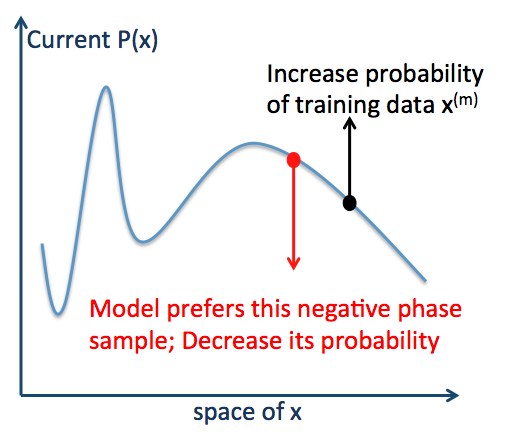
\includegraphics[scale=0.4]{figs/contrastive_divergence}}
\end{frame}

%% SUBSECTION%%%%%
\subsection[DBN]{Stacking RBMs to form Deep Belief Nets}

%%%%%
\begin{frame}
\frametitle{Deep Belief Nets (DBN) = Stacked RBM}
\begin{columns}
\begin{column}{0.5\textwidth}
\begin{center}
\begin{tikzpicture}[-,>=stealth',shorten >=1pt,auto,node distance=3cm,
  thick,main node/.style={circle,fill=blue!20,draw,font=\sffamily\Large\bfseries}]

  \node[main node] (x1) at (0,0) {$x_1$};
  \node[main node] (x2) at (2,0) {$x_2$};
  \node[main node] (x3) at (4,0) {$x_3$};
  \node[main node] (h1) at (0,2) {$h_1$};
  \node[main node] (h2) at (2,2) {$h_2$};
  \node[main node] (h3) at (4,2) {$h_3$};
  \node[main node] (h'1) at (0,4) {$h'_1$};
  \node[main node] (h'2) at (2,4) {$h'_2$};
  \node[main node] (h'3) at (4,4) {$h'_3$};
  \node[main node] (h''1) at (0,6) {$h''_1$};
  \node[main node] (h''2) at (2,6) {$h''_2$};
  \node[main node] (h''3) at (4,6) {$h''_3$};
  \node at (5.1,1) {Layer1 RBM};
  \node at (5.1,3) {Layer2 RBM};
  \node at (5.1,5) {Layer3 RBM};


  \path[every node/.style={font=\sffamily\small}]
    (x1) edge node {} (h1)
    (x1) edge node {} (h2)
    (x1) edge node {} (h3)
    (x2) edge node {} (h1)
    (x2) edge node {} (h2)
    (x2) edge node {} (h3)
    (x3) edge node {} (h1)
    (x3) edge node {} (h2)
    (x3) edge node {} (h3)
    (h1) edge node {} (h'1)
    (h1) edge node {} (h'2)
    (h1) edge node {} (h'3)
    (h2) edge node {} (h'1)
    (h2) edge node {} (h'2)
    (h2) edge node {} (h'3)
    (h3) edge node {} (h'1)
    (h3) edge node {} (h'2)
    (h3) edge node {} (h'3)
    (h'1) edge node {} (h''1)
    (h'1) edge node {} (h''2)
    (h'1) edge node {} (h''3)
    (h'2) edge node {} (h''1)
    (h'2) edge node {} (h''2)
    (h'2) edge node {} (h''3)
    (h'3) edge node {} (h''1)
    (h'3) edge node {} (h''2)
    (h'3) edge node {} (h''3)
    ;

\end{tikzpicture}
\end{center}
\end{column}
\begin{column}{0.5\textwidth}
\bi
\item DBN defines a probabilistic generative model $p(x)=\sum_{h,h',h''}p(x|h)p(h|h')p(h',h'')$
 (top 2 layers is interpreted as a RBM; lower layers are directed sigmoids)\pause
\item Stacked RBMs can also be used to initialize a Deep Neural Network (DNN)
\ei
\end{column}
\end{columns}
\end{frame}



%%%%%%%%%%%%%
\begin{frame}
\frametitle{Generating Data from a Deep Generative Model}
After training on 20k images, the generative model of \cite{salakhutdinov09dbm}* can generate random images (dimension=8976) that are amazingly realistic!
\vspace{1cm} 
\centerline{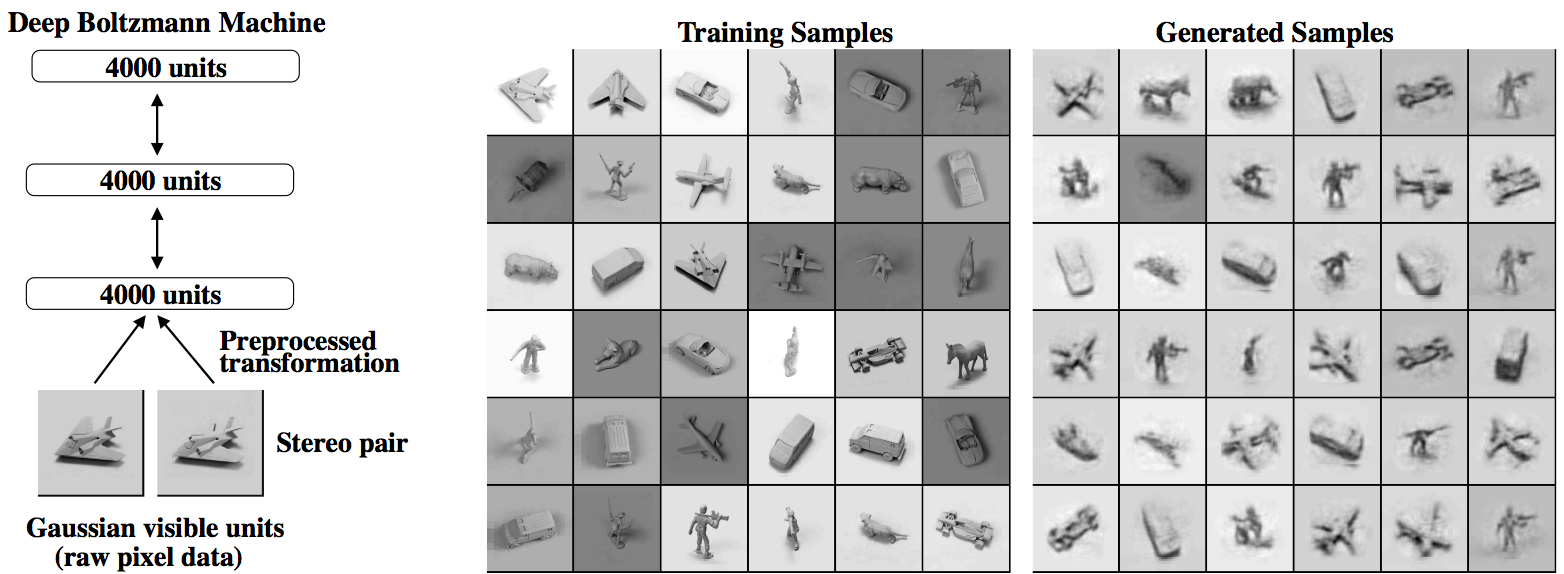
\includegraphics[scale=0.2]{figs/dbm_generation}}
\blfootnote{This model is a Deep Boltzmann Machine (DBM), different from Deep Belief Nets (DBN) but also built by stacking RBMs.}
\end{frame}

%%%%%%%%%%%%%
\begin{frame}
\frametitle{Summary: Things to remember about DBNs}
\be
\item Layer-wise pre-training is the innovation that rekindled interest in deep architectures. \pause
\item Pre-training focuses on optimizing likelihood on the data, not the target label. First model $p(x)$ to do better $p(y|x)$. \pause
\item Why RBM? $p(h|x)$ is tractable, so it's easy to stack.\pause
\item RBM training can be expensive. Solution: contrastive divergence\pause
\item DBN formed by stacking RBMs is a probabilistic generative model
\ee
\end{frame}

%SECTION%%%%%%%%%%%%%%%%%%%
\section[Approach 2: Stacked Auto-Encoders]{Approach 2: Stacked Auto-Encoders \cite{bengio06greedy}}
%%%%%%%%%%%%%%%%%%%%

%% SUBSECTION%%%%%
\subsection[Auto-Encoders]{Auto-Encoders}

\begin{frame}
\frametitle{Auto-Encoders: simpler alternatives to RBMs}

\begin{center}
\begin{tikzpicture}[->,>=stealth',shorten >=1pt,auto,node distance=3cm,
  thick,main node/.style={circle,fill=blue!20,draw,font=\sffamily\Large\bfseries}]

  \node[main node] (x1) at (0,0) {$x_1$};
  \node[main node] (x2) at (2,0) {$x_2$};
  \node[main node] (x3) at (4,0) {$x_3$};
  \node[main node] (h1) at (1,2) {$h_1$};
  \node[main node] (h2) at (3,2) {$h_2$};
  \node[main node] (h'1) at (0,4) {$x'_1$};
  \node[main node] (h'2) at (2,4) {$x'_2$};
  \node[main node] (h'3) at (4,4) {$x'_3$};
  \node at (7,1) {Encoder: $h =\sigma(Wx+b)$ };
  \node at (7,3) {Decoder: $x' =\sigma(W'h+d)$};


  \path[every node/.style={font=\sffamily\small}]
    (x1) edge node {} (h1)
    (x1) edge node {} (h2)
    (x2) edge node {} (h1)
    (x2) edge node {} (h2)
    (x3) edge node {} (h1)
    (x3) edge node {} (h2)
    (h1) edge node {} (h'1)
    (h1) edge node {} (h'2)
    (h1) edge node {} (h'3)
    (h2) edge node {} (h'1)
    (h2) edge node {} (h'2)
    (h2) edge node {} (h'3);

\end{tikzpicture}
\end{center}
\pause
Encourage $h$ to give small reconstruction error:
	\bi
	\item e.g. $Loss = \sum_m || x^{(m)} - DECODER(ENCODER(x^{(m)})) ||^2 $\pause
	\item Reconstruction: $x' =\sigma(W'\sigma(Wx+b)+d)$\pause
	\item This can be trained with the same Backpropagation algorithm for 2-layer nets, with $x^{(m)}$ as both input and output
	\ei
\end{frame}



%%%%%%%%%
\begin{frame}
\frametitle{Stacked Auto-Encoders (SAE)}
\bi 
\item The encoder/decoder gives same form $p(h|x)$, $p(x|h)$ as RBMs, so can be stacked in the same way to form Deep Architectures
\pause
\begin{center}
\scalebox{0.7}{\begin{tikzpicture}[->,>=stealth',shorten >=1pt,auto,node distance=3cm,
  thick,main node/.style={circle,fill=blue!20,draw,font=\sffamily\Large\bfseries}]

  \node[main node] (x1) at (0,0) {$x_1$};
  \node[main node] (x2) at (2,0) {$x_2$};
  \node[main node] (x3) at (4,0) {$x_3$};
  \node[main node] (x4) at (6,0) {$x_4$};
  \node[main node] (h1) at (1,2) {$h_1$};
  \node[main node] (h2) at (3,2) {$h_2$};
  \node[main node] (h3) at (5,2) {$h_3$};
  \node[main node] (h'1) at (2,4) {$h'_1$};
  \node[main node] (h'2) at (4,4) {$h'_2$};
  \node[main node] (y) at (3,6) {$y$};
  \node at (7,1) {Layer1 Encoder};
  \node at (7,3) {Layer2 Encoder};
  \node at (7,5) {Layer3 Encoder};


  \path[every node/.style={font=\sffamily\small}]
    (x1) edge node {} (h1)
    (x1) edge node {} (h2)
    (x1) edge node {} (h3)
    (x2) edge node {} (h1)
    (x2) edge node {} (h2)
    (x2) edge node {} (h3)
    (x3) edge node {} (h1)
    (x3) edge node {} (h2)
    (x3) edge node {} (h3)
    (x4) edge node {} (h1)
    (x4) edge node {} (h2)
    (x4) edge node {} (h3)
    (h1) edge node {} (h'1)
    (h1) edge node {} (h'2)
    (h2) edge node {} (h'1)
    (h2) edge node {} (h'2)
    (h3) edge node {} (h'1)
    (h3) edge node {} (h'2)
    (h'1) edge node {} (y)
    (h'2) edge node {} (y)
  
    ;
\end{tikzpicture}}
\end{center}

\pause
\item Unlike RBMs, Auto-encoders are deterministic. 
	\bi
	\item $h =\sigma(Wx+b)$, not $p(h=\{0,1\}) =\sigma(Wx+b)$\pause
	\item Disadvantage: Can't form deep generative model
	\item Advantage: Fast to train, and useful still for Deep Neural Nets
	\ei
\ei

\end{frame}

%%%%%%%%%%%%%%
\begin{frame}
\frametitle{Many Variants of Auto-Encoders}
\bi 
\item Enforce compression to get latent factors (lower dimensional $h$) \pause
\item Linear encoder/decoder with squared reconstruction error learns same subspace of PCA \cite{bourlard88auto} \pause
\item Enforce sparsity and over-complete representations (high dimensional $h$) \cite{ranzato06sparse}
\item Enforce binary hidden layers to build hash codes \cite{salakhutdinov07hash}
\item Incorporate domain knowledge, e.g. denoising auto-encoders \cite{vincent10denoise}
\ei
\end{frame}


%% SUBSECTION%%%%%
\subsection[Denoising Auto-Encoders]{Denoising Auto-Encoders}

\begin{frame}
\frametitle{Denoising Auto-Encoders}

\begin{center}
\begin{tikzpicture}[->,>=stealth',shorten >=1pt,auto,node distance=3cm,
  thick,main node/.style={circle,fill=blue!20,draw,font=\sffamily\Large\bfseries}]

  \node[main node] (x1) at (0,0) {$\tilde{x_1}$};
  \node[main node] (x2) at (2,0) {$\tilde{x_2}$};
  \node[main node] (x3) at (4,0) {$\tilde{x_3}$};
  \node[main node] (h1) at (1,2) {$h_1$};
  \node[main node] (h2) at (3,2) {$h_2$};
  \node[main node] (h'1) at (0,4) {$x'_1$};
  \node[main node] (h'2) at (2,4) {$x'_2$};
  \node[main node] (h'3) at (4,4) {$x'_3$};
  \node at (7,0) {$\tilde{x} = x + $ noise};
  \node at (7,1) {Encoder: $h =\sigma(W\tilde{x}+b)$ };
  \node at (7,3) {Decoder: $x' =\sigma(W'h+d)$};


  \path[every node/.style={font=\sffamily\small}]
    (x1) edge node {} (h1)
    (x1) edge node {} (h2)
    (x2) edge node {} (h1)
    (x2) edge node {} (h2)
    (x3) edge node {} (h1)
    (x3) edge node {} (h2)
    (h1) edge node {} (h'1)
    (h1) edge node {} (h'2)
    (h1) edge node {} (h'3)
    (h2) edge node {} (h'1)
    (h2) edge node {} (h'2)
    (h2) edge node {} (h'3)
    ;

\end{tikzpicture}
\end{center}

\be
\item Perturb input data $x$ to $\tilde{x}$ using invariance from domain knowledge. 
\item Train weights to reduce reconstruction error with respect to original input: $||x-x'||$
\ee
\end{frame}


\begin{frame}
\frametitle{Denoising Auto-Encoders}
\bi
\item Example: Randomly shift, rotate, and scale input image; add Gaussian or salt-and-pepper noise.
\item A "2" is a "2" no matter how you add noise, so the auto-encoder will be forced to cancel the variations that are not important. 
\ei
\centerline{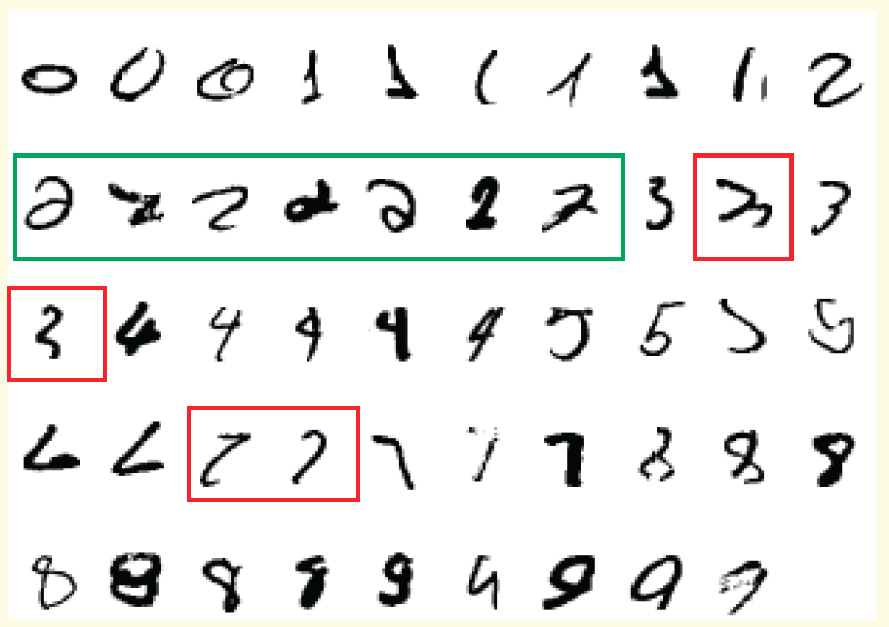
\includegraphics[scale=0.19]{figs/digit2}}
\end{frame}

%%%%%%%%%%%%%%%%%%%%%%%%%%%%%%%%%%%%%%
\begin{frame}
\frametitle{Summary: things to remember about SAE}
\be
\item Auto-Encoders are cheaper alternatives to RBMs.
	\bi
	\item Not probabilistic, but fast to train using Backpropagation or SGD
	\ei
\pause
\item Auto-Encoders learn to "compress" and "re-construct" input data. Again, the focus is on modeling $p(x)$ first.  \pause
\item Many variants, some provide ways to incorporate domain knowledge.
\ee
\end{frame}



%% SECTION%%%%%
\section{Discussions}
%%%%%%%%%%%%%%%

\subsection[Why]{Why it works, when it works, and the bigger picture}

\begin{frame}
\frametitle{Why does Layer-wise Pre-Training work?}
One Hypothesis \cite{bengio09book,erhan10pretrain}:
\bi
\item A deep net can fit the training data in many ways (non-convex):
	\be
	\item By optimizing upper-layers really hard
	\item By optimizing lower-layers really hard
	\ee
\pause
\item Top-down vs. Bottom-up information
	\be
	\item Even if lower-layers are random weights, upper-layer may still fit well. But this might not generalize to new data
	\item Pre-training with objective on $P(x)$ learns more generalizable features
	\ee
\pause
\item Pre-training seems to help put weights at a better local optimum
\ei
\centerline{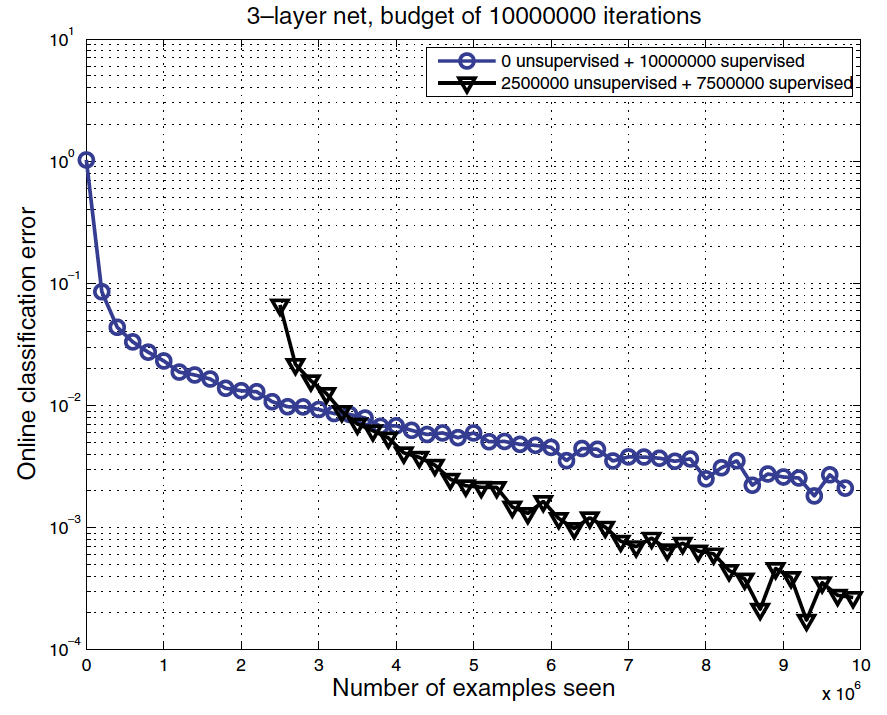
\includegraphics[scale=0.18]{figs/pretrain_vs_none}}
\end{frame}

\begin{frame}
\frametitle{Is Layer-wise Pre-Training always necessary?}
\pause
Answer in 2006: Yes!

\pause
Answer in 2014: No!
\be
\item If initialization is done well by design (e.g. sparse connections and convolutional nets), maybe won't have vanishing gradient problem\pause
\item If you have an extremely large datasets, maybe won't overfit. (But maybe that also means you want an ever deeper net)\pause
\item New architectures are emerging:
	\bi
	\item Stacked SVM's with random projections \cite{vinyals12}
	\item Sum-Product Networks \cite{poon11sumproduct}
	\ei
\ee 
\end{frame}

\begin{frame}
\frametitle{Connections with other Machine Learning concepts}
\bi
\item A RBM is like a product-of-expert model and forms a distributed representation of the data
	\bi
	\item Compared with clustering (which compresses data but loses information), distributed representations (multi-clustering) are richer representations 
	\item Like a mixture model with $2^n$ hidden components $p(x)=\sum_h p(h)p(x|h)$, but much more compact
	\ei
\pause
\item Neural Net as kernel for SVM \cite{li05mlp} and SVM training for Neural Nets \cite{collobert04links}
\pause
\item Decision trees are deep (but no distributed representation). Random forests are both deep and distributed. They do well in practice too!
\pause
\item Philosophical connections to:
	\bi
	\item Semi-supervised Learning: exploit both labeled and unlabeled data
	\item Curriculum Learning: start on easy task, gradually level-up
	\item Multi-task Learning: learn and share sub-tasks
	\ei
\ei
\end{frame}


%%%%%%%%%%%%%%%%
\begin{frame}
\frametitle{History}
\begin{itemize}
\item {\color{blue} Early days of AI.} Invention of artificial neuron \cite{mcculloch43} \& perceptron \cite{rosenblatt58} \pause
\item {\color{red} AI Winter.} \cite{minsky69} showed perceptron only learns linearly separable concepts \pause
\item {\color{blue} Revival in 1980s:} Multi-layer Perceptrons (MLP) and Back-propagation \cite{rumelhart86} \pause
\item {\color{red} Other directions (1990s - present):} SVMs, Bayesian Networks \pause
\item {\color{blue} Revival in 2006:} Deep learning \cite{hinton06dbn} \pause
\item {\color{blue} Successes in applications:} Speech at IBM/Toronto \cite{sainath11deep}, Microsoft \cite{dahl12deep}.  Vision at Google/Stanford \cite{le12highlevel}  
\end{itemize}
\end{frame}


\begin{frame}[allowframebreaks]
\frametitle{References}
\bibliographystyle{apalike}
\bibliography{mybib}
\end{frame}

\end{document}
